%% LaTeX-Beamer template for KIT design
%% by Erik Burger, Christian Hammer
%% title picture by Klaus Krogmann
%%
%% version 2.1
%%
%% mostly compatible to KIT corporate design v2.0
%% http://intranet.kit.edu/gestaltungsrichtlinien.php
%%
%% Problems, bugs and comments to
%% burger@kit.edu

\documentclass[18pt]{beamer}
\usepackage[utf8x]{inputenc}
\usepackage{units}
\usepackage{booktabs}

%% CUSTOM
\usepackage{amsmath}
\usepackage{algpseudocode}

%% Definitions
\DeclareMathOperator{\div2}{div}
\renewcommand{\algorithmicrequire}{\textbf{Input:}}
\renewcommand{\algorithmicensure}{\textbf{Output:}}
\algnewcommand\algorithmicto{\textbf{to}}
\algrenewtext{For}[3]{\algorithmicfor\ $#1 \gets #2$ \algorithmicto\ $#3$ \algorithmicdo}
\algnewcommand\algorithmicod{\textbf{od}}
\algrenewtext{EndWhile}{\algorithmicod}
\algrenewtext{EndFor}{\algorithmicod}
%\AtBeginSection[]{%
%\begin{frame}<beamer> % do nothing in handouts
%    \frametitle{Überblick}
%    \tableofcontents[sectionstyle=show/shaded,
%    subsectionstyle=show/show/hide]
%\end{frame}
%}
%\AtBeginSubsection[]{%
%\begin{frame}<beamer> % do nothing in handouts
%    \frametitle{Überblick}
%    \tableofcontents[sectionstyle=show/shaded,
%    subsectionstyle=show/shaded/hide]
%\end{frame}
%}

%% SLIDE FORMAT

% use 'beamerthemekit' for standard 4:3 ratio
% for widescreen slides (16:9), use 'beamerthemekitwide'

\usepackage{templates/beamerthemekit}
%\usepackage{templates/beamerthemekitwide}

 %% TITLE PICTURE

 % if a custom picture is to be used on the title page, copy it into the 'logos'
 % directory, in the line below, replace 'mypicture' with the 
 % filename (without extension) and uncomment the following line
 % (picture proportions: 63 : 20 for standard, 169 : 40 for wide
 % *.eps format if you use latex+dvips+ps2pdf, 
 % *.jpg/*.png/*.pdf if you use pdflatex)


 \titleimage{banner}
 
 
%% Define some colors:
\definecolor{darkblue}{rgb}{0,0,.5}
\definecolor{darkgreen}{rgb}{0,.5,0}

 %% TITLE LOGO

 % for a custom logo on the front page, copy your file into the 'logos'
 % directory, insert the filename in the line below and uncomment it

\titlelogo{logo_150x150}
 
 % (*.eps format if you use latex+dvips+ps2pdf,
 % *.jpg/*.png/*.pdf if you use pdflatex)
 
 %% TikZ INTEGRATION
 
 % use these packages for PCM symbols and UML classes
 % \usepackage{templates/tikzkit}
 % \usepackage{templates/tikzuml}
 
 % the presentation starts here
 
\author{Dominik Muth - dominik.muth@student.kit.edu}
\institute{Institut f\"ur Informatik}


\title[Tutorium 4]{GBI Tutorium Nr. $2^5$}
\subtitle{Tutorium 4}
\date{7. November 2012}

% Bibliography



\begin{document}

	%title page
	\begin{frame}
		\titlepage
	\end{frame}

	%table of contents
	\begin{frame}{Outline/Gliederung}
		\tableofcontents
	\end{frame}
	
	
	\section{Feedback und Folien}
	\begin{frame} {Feedback und Folien}
		\begin{center}
			
\includegraphics[scale=.6]{graphics/03/feedback.png}\\
			\small domi-individual.bplaced.de/tut/
		\end{center}
	\end{frame}
	
	
	\section{\"Ubungsblatt 3}
	\begin{frame} {Übungsblatt 3}
		\begin{block} {Aufgabe 3.3 a)}
			$|L_1^2| = |L_1 \times L_1|$
		\end{block}
		\pause
		\begin{block} {Aufgabe 3.3 c)}
			$(L_1 \cup L_2)^* = (L_1^* \cdot L_2^*)^*$
		\end{block}
	\end{frame}	
		
	
	
	
	\section{Wiederholung} 
	\begin{frame} {Wiederholung - Quiz}
		\begin{itemize}
			\item $A^*$ ist eine formale Sprache! 
			\only<2-> {\color{darkgreen}$\surd$}\\
			\color{black}
			\item $(L_1 \cdot L_2)^* = L_1^* \cdot L_2^*$
			\only<3-> {\color{red}$X$}\\
			\color{black}
			\item $f(x) = x^3-x^2$ ist rechtstotal für $x, f(x) \in \mathbb{R}$.
			\only<4-> {\color{darkgreen}$\surd$}\\
			\color{black}
			\item Eine bijektive Relation ist eine Funktion.
			\only<5-> {\color{darkgreen}$\surd$}\\
			\color{black}
			\item Wenn $f: A \rightarrow B$ injektiv $\Rightarrow f^{-1}$ ist surjektiv.
			\only<6-> {\color{red}$X$}\\
			\color{black}
			\item $A\Rightarrow B \Leftrightarrow \neg B \Rightarrow \neg A$
			\only<7-> {\color{darkgreen}$\surd$}\\
		\end{itemize}
	\end{frame}
	
	
	
	\begin{frame} {Wiederholung - Aufgaben}
		\begin{itemize}
			\item Schreiben sie die Injektivität als Prädikatenlogische Formel.
			\pause
			\item Es sei $L \subseteq A^*$ eine formale Sprache. Beweisen oder widerlegen Sie:\\
			$L^+ \cdot L^+ \subseteq L^+$
		\end{itemize}
	\end{frame}
	
	
	
	\begin{frame} {Wiederholung}
		\begin{block}{Induktion}
			Alice und Bob feiern ihren Hochzeitstag. Auf ihrer Party befinden sich $n \in \mathbb{N}_+$ Paare.
			Dabei begrüßen sich alle Paare mit Ausnahme des eigenen Partners.\\
			\vspace{10pt}
			a) Geben Sie die Anzahl der Begrüßungen $x_i$ für $i \in \{1,2,3,4,5\}$ Paare an.\\
			\vspace{10pt}
			b) Stellen Sie für $x_n$ eine geschlossene Formel (d.h. einen arithmetischen Ausdruck, in dem nur Zahlen, n und die Grundrechenarten vorkommen) auf.\\
			\vspace{10pt}
			c) Beweisen Sie Ihre Aussage aus Teilaufgabe b) durch vollständige Induktion
		\end{block}
	\end{frame}
	
	
	\section{Pseudocode}
	\begin{frame}{Pseudocode}
		\begin{block} {Was ist Pseudocode}
			Pseudocode ist Programmcode, der zur Darstellung von Algorithmen verwendet wird.\\
		\end{block}
		
		\begin{block} {Konvention in GBI}
			\begin{itemize}
				\item Zuweisung: $x \leftarrow 42$
				\pause
				\item Kommentare: $//$Kommentar
				\pause
				\item Schleifen: \\
				$for$ $i \leftarrow 0$ $to$ $42 do$ $.........$ $od$\\
				$while$ $i < 42$ $do$ $.........$ $od$
				\pause
				\item Abfrage: $if$ $i = 42 then ....... endif$
			\end{itemize}			 
		\end{block}
	\end{frame}
	
	
	
	\section{div / mod}
	\begin{frame} {div / mod}
		\begin{block} {Erläuterung div}
			x div y entspricht der Ganzzahldivision ohne Rest:\\ $\lfloor \frac{x}{y} \rfloor$\\
			Beispiel: $14$ $div$ $3 = 2$
		\end{block}
		\begin{block} {Erläuterung mod}
			x mod y entspricht dem Rest der Ganzzahldivision.\\
			Beispiel:\\
			$5$ $mod$ $3 = 2$\\
			Mod lässt sich auch durch $\cdot$, $-$ und div darstellen:\\
			$x$ $mod$ $y$ = $x - (y \cdot (x$ $div$ $y))$
		\end{block}
	\end{frame}
	
	
	\begin{frame} {Übung}
		\begin{block}{}
		Fülle folgende Tabelle aus:\\
		\vspace{10pt}
			\begin{tabular}{l|cccccccccccc}
				$x$ & 0 & 1 & 2 & 3 & 4 & 5 & 6 & 7 & 8 & 9 & 10 & 11\\
				$x$ \textbf{div} $4$ & & & & & & & & & & & & \\
				$4(x$ \textbf{div} $4)$ & & & & & & & & & & & & \\
				$x$ \textbf{mod} $4$ & & & & & & & & & & & & \\
			\end{tabular}
		\end{block}
	\end{frame}
	
	
	\section{Algorithmen}
	\begin{frame} {Algorithmen}
		\begin{block} {Eigenschaften}
			Ein Algorithmus...\\
			\begin{itemize}
				\item hat eine endliche Beschreibung,
				\pause
				\item besteht aus elementaren Anweisungen,
				\pause
				\item ist deterministisch,
				\pause
				\item gibt endliche Ausgabe auf endliche Eingabe aus,
				\pause
				\item hat endlich viele Schritte,
				\pause
				\item ist skalierbar
				\pause
				\item und ist nachvollziehbar
			\end{itemize}
		\end{block}
	\end{frame}
	
	
	\subsection{Schleifen}
	\begin{frame}{Schleifen}
		\begin{block}{while Schleife}
			Eine while Schleife wiederholt etwas, solange eine Bedingung erfüllt ist.\\
			Pseudocode: \textbf{while} $x > 1$ \textbf{do} .... \textbf{od}\\
			Jave: while($x > 1$) $\{$ .... $\}$
		\end{block}	
		
			
		\begin{block}{do while Schleife}
			Eine do while Schleife tut erst etwas, prüft danach, ob die Bedingung erfüllt ist und wiederholt dann den schleifenrumpf.\\
			Pseudocode:  \textbf{do} .... \textbf{od} \textbf{while} $x > 1$\\
			Jave: do $\{$ .... $\}$while($x > 1$)
		\end{block}		
	\end{frame}
	
	
	\begin{frame}{Schleifen}
		\begin {exampleblock}{Beispiel 1}
     		\begin{algorithmic}
                \Require $x \in \mathbb{N}_+$
                \State $i \gets 0$
                \While{$x > 1$}
                    \State $x\gets x \div2 2$
                    \State $i\gets i + 1$
                \EndWhile
                \Ensure $i$
        	\end{algorithmic}
        \end{exampleblock}
	\end{frame}
	

	\begin{frame}{Schleifen}
		\begin{exampleblock}{Beispiel 2}
			\begin{algorithmic}
				\State $k \gets 0$
				\For{i}{0}{20}
					\State $k\gets k+i$
				\EndFor
				\Ensure $k$
			\end{algorithmic}
		\end{exampleblock}
	\end{frame}
	
	\begin{frame}{Schleifen}
    	\begin{exampleblock}{Beispiel 3}
        	Gegeben sei ein Wort $w$ der Länge $\left| w\right| = n$. 
        	Das Array $W$ hat an $i$-ter Stelle den $i$-ten Buchstabe von $w$.
        	$w$ ist $\epsilon$-frei.
            \begin{algorithmic}
                \State $c \gets 0$
                \For{i}{0}{n-1}
                	\If{$A[i\,] = $'x'}
                		\State $c \gets c+1$
    				\EndIf
                \EndFor
                \Ensure $c$
            \end{algorithmic}
    	\end{exampleblock}
	\end{frame}
	

	\begin{frame}{Schleifen}
    	\begin{exampleblock}{Übung 1, Winter 2008/2009}
        	Es sei $A$ ein Alphabet.\\
        	Schreiben Sie einen Algorithmus auf, der folgendes leistet: 
        	Als Eingaben erhält er ein Wort $w$ über $A$ und zwei Symbole 
        	$x \in A$ und $y \in A$. 
        	Am Ende soll eine Variable $r$ den Wert $0$ oder $1$ haben,
        	und zwar soll gelten:\\
        	\begin{align*}
            	r = \begin{cases} 1 & \text{falls irgendwo in w 
            	direkt hintereinander erst $x$ dann $y$ vorkommt}\\ 
            	0 &\text{sonst}\end{cases}
        	\end{align*}
        	Benutzen Sie zum Zugriff auf das $i$-te Symbol von $w$ 
        	die Schreibweise $w\left( i\right)$. 
        	Formulieren Sie den Algorithmus mit Hilfe einer for-Schleife.
    	\end{exampleblock}
	\end{frame}
	
	
	\section{Schleifeninvarianz}
	\begin{frame}{Schleifeninvarianz}
		\begin{block}{Definition}
			Die Schleifeninvarianz bezeichnet eine 
			Bedingung innerhalb einer Schleife, 
			welche bei jedem Schleifendurchlauf gültig ist.
		\end{block}
	\end{frame}


	\begin{frame}{Schleifeninvarianz}
		\begin{block}{Wofür?}
			Mit Schleifeninvarianten lässt sich die Korrektheit von Algorithmen beweisen.
		\end{block}
		
		\begin{block}{Wie}
			Mit vollständiger Induktion
		\end{block}
	\end{frame}
	
	
	\begin{frame}{Schleifeninvarianz}
   		\begin{block}{Beispiel}
            \begin{algorithmic}
                \Require $a, b \in \mathbb{N}_0$
                \State $S \gets a$
                \State $Y \gets b$
                \For{i}{0}{b-1}
                    \State $ S \gets S - 1$
                    \State $Y \gets Y -1$
                \EndFor
                \Ensure $S$
            \end{algorithmic}
    	\end{block}
    	
    	\pause
    	
    	\begin{exampleblock}{Übung}
        	Algorithmus mit $a = 3$ und $b = 4$ ausprobieren und Werte für $S$ 
        	und $Y$ bei jedem Schleifendurchlauf finden.
    	\end{exampleblock}
	\end{frame}
	
	
	\begin{frame}{Schleifeninvarianz}
		\begin{exampleblock}{Übung}
			Gegeben sei folgendes Programmstück:\\
			\begin{algorithmic}
				\State $X_0 \gets 2$
				\State $Y_0 \gets 5$
				\For{i}{0}{n}
					\State $j \gets i$
					\State $Y_{j+1} \gets 5Y_j - 6X_j$
					\State $X_{j+1} \gets Y_j$
				\EndFor
			\end{algorithmic}
			\vspace{10pt}
			Beweisen Sie die Korrektheit der folgenden Aussage:\\
			$Y_j=2^{j+1}+3^{j+1} \land X_j = 2^j + 3^j$
		\end{exampleblock}
	\end{frame}
	
	
	
	\section{Fragen}
	\begin{frame} {Fragen}
		\begin{itemize}
			\item Fragen zum Stoff?
			\item Fragen zum n\"achsten \"Ubungsblatt?
			\item Generelle Fragen?
		\end{itemize}
	\end{frame}

		
	\begin{frame} {EOF}
		\begin{center}
			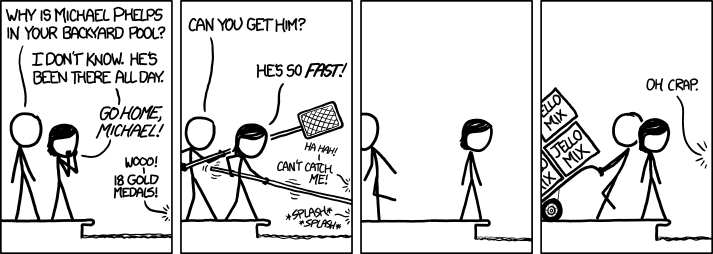
\includegraphics[scale=0.4]{graphics/eof4.png}\\
			\tiny $source: http://imgs.xkcd.com/comics/michael_phelps.png$
		\end{center}
	\end{frame}

\end{document}
